\documentclass[5p]{elsarticle}

\usepackage{amsmath}
\usepackage{booktabs}
\usepackage{graphicx}
\usepackage{listings}
\usepackage{natbib}
\usepackage{soul}  % highlighting text
\usepackage{xcolor}

\definecolor{mygreen}{rgb}{0,0.6,0}
\definecolor{mygray}{rgb}{0.5,0.5,0.5}
\definecolor{mymauve}{rgb}{0.58,0,0.82}

\lstset{ 
  backgroundcolor=\color{white},   % choose the background color; you must add \usepackage{color} or xcolor 
  basicstyle=\tiny,        % the size of the fonts that are used for the code
  breakatwhitespace=false,         % sets if automatic breaks should only happen at whitespace
  breaklines=true,                 % sets automatic line breaking
  captionpos=b,                    % sets the caption-position to bottom
  commentstyle=\color{mygreen},    % comment style
  frame=single,	                   % adds a frame around the code
  keepspaces=true,                 % keeps spaces in text, useful for keeping indentation of code (possibly needs columns=flexible)
  keywordstyle=\color{blue},       % keyword style
  numbers=left,                    % where to put the line-numbers; possible values are (none, left, right)
  numbersep=5pt,                   % how far the line-numbers are from the code
  numberstyle=\tiny\color{mygray}, % the style that is used for the line-numbers
  rulecolor=\color{black},         % if not set, the frame-color may be changed on line-breaks within not-black text (e.g. comments (green here))
  stepnumber=1,                    % the step between two line-numbers. If it's 1, each line will be numbered
  stringstyle=\color{mymauve},     % string literal style
  tabsize=2,	                   % sets default tabsize to 2 spaces
}

\hfuzz=5pt

\title{Enabling Advanced Building Simulation Workflows with APIs and Plugins} 
\author{Edwin Lee and Matt Mitchell}
\date{\today}

\begin{document}
  
 \begin{abstract}
Admirable goals for energy efficiency and grid interactivity require a deeper understanding of the interactions between buildings and the electric grid.  Whole-building energy simulation has been used for decades to answer some of the relevant research questions, and over time, the questions have evolved to become more complicated and complex.  The questions of today regarding grid-interactive efficient buildings require incredibly detailed calculations that can be deployed in broad, rapid ways. For two decades, the program building energy simulation engine “EnergyPlus” has been used by thousands of engineers, architects and designers to perform building energy analysis. While it has been effective, answering today’s questions requires new capabilities that don’t just add more physics to the model, but open the door for a broad user base to add their own detailed modeling capabilities in a very straightforward way.  In this paper, new workflows are enabled around EnergyPlus by exposing EnergyPlus functionality through a new API, and allowing EnergyPlus to call out to user-defined Python code.

\hl{This is part of a two paper submission related to the EnergyPlus API.  In this paper, the API is described and justified, while in the second companion paper, applications of this API are exercised with advanced control strategies.}
 \end{abstract}

 \maketitle
 
 \section{Background}

The simulation of building physics has been around for many decades, with countless variations in accuracy and flexibility.  In the 1990s, the United States Department of Energy set out to create a state of the art flagship simulation engine, which was ultimately named EnergyPlus and released around the turn of the century \cite{Crawley2001}.  Since that time, EnergyPlus has evolved in many ways, some very major, with Table~\ref{table:background:events} capturing some of the major changes to the tool.

\begin{table}[h!]
\begin{center}
\caption{Major related events in EnergyPlus development}
\begin{tabular}{@{}ll@{}}
\toprule
Year         & Event                               \\ 
\midrule
1999 or 2000 & Initial release of EnergyPlus       \\
2009         & User defined controls (EMS)         \\
2011?        & External interface for cosimulation \\
2014         & Conversion from Fortran to C++      \\ 
\bottomrule
\end{tabular}
\label{table:background:events}
\end{center}
\end{table}

Each of the events listed in Table~\ref{table:background:events} were critical in improving the usability and/or accuracy of the tool, thus playing a role in establishing the current state of the program.  Recent releases of the tool have achieved around 40,000 direct downloads, plus many thousand more uses as it is packaged with software development kits like OpenStudio as well as with other commercial graphical interfaces. 

  \subsection{User Defined Controls}
The Energy Management System (EMS) in EnergyPlus allows users to read simulation data, and actuate simulation controls--according to their own custom logic--at a selected frequency within a running simulation.  This was ultimately extended to not only allow users to write custom control logic, but also to define custom component models entirely.  This was a major advancement that allowed users to fill in the gaps of the built-in EnergyPlus controls and component models, to perform simulations that involved niche, obscure, or cutting edge technologies and controls that are not pre-compiled with the EnergyPlus release.  These have been exercised by developers. \cite{Dutton2012, Jones2013, Sardoueinasab2019, Sardoueinasab2020} At the time of implementation, EnergyPlus was still in the adolescent phase of development, and was viewed primarily as a research-oriented tool.  The addition of a user defined language supported the research interest for simulating novel control strategies and technologies, but also ensured that companies could simulate their as-built technologies without having to contribute control logic back into the original Fortran codebase.  This spurred interest in the tool from new industry partners and was critical for moving EnergyPlus towards achieving widespread adoption.  As capabilities built around the Energy Management System evolved, the name became less representative of the true power.  With the ability to actuate thousands of controls and settings in a running simulation, the system became more of a generic plugin system which allows simulation of user-specified components and controls.  However, with all that power, the EMS code was still restricted in a few primary ways:
\begin{itemize}
  \item The language -- EnergyPlus Runtime Language is a completely custom language with no support system outside of EnergyPlus itself
  \item Language features -- features were limited to a small set of language constructs and data types to avoid having to maintain a complex language
  \item Functionality implementation -- user-defined functionality must be written directly into the context of the input file syntax, IDF, which makes the resulting code clumsy to manage
  \item Program debugging -- the resulting program involves parsing through stack evaluation files which easily enter into the gigabytes of data, with no easy way to limit outputs to specific times/variables
\end{itemize}

Even with these limitations, the Energy Management System was an impressive feature and helped EnergyPlus expand further into research and development, but also into commercial opportunities.

  \subsection{External Interface}
The external interface feature of EnergyPlus was an attempt to create a form of API to allow other tools to communicate with EnergyPlus.  The specifics of this system are available in literature \cite{Nouidui2014}, but it can be summarized as a socket-based approach to allowing tools to communicate with a running simulation (VERIFY THIS).  This system was used by the BCVTB \cite{Pang2011} and was the first attempt at exposing the core of EnergyPlus to other tools.  The real problem of this is that wiring up new capabilities requires expertise in multiple domains: computer science and software development to set up these tools and programs, but then also the mechanical and building science expertise to make engineering judgments during model development and results evaluation.  This greatly limited the number of users who could make use of this development.

  \subsection{Conversion from Fortran to C++}
At the birth of EnergyPlus, Fortran 95 provided far and above the most state of the art programming capabilities for a numerical simulation tool.  Capabilities such as dynamically allocating user defined derived types allowed the program to be computationally efficient while benefiting from the memory management of the Fortran language and runtime.  Fortran was the right choice for creating the simulation tool, and persisted as the best choice of language for well over a decade. In that time, the C++ language gained popularity while Fortran fell behind.  The ability to do commonplace modern coding practices in Fortran justifies a journal paper \cite{Oezturan2015}.  While the C++ language is missing some features such as built-in multi-dimensional array support, the developer base and community surrounding it opens up access to many modern libraries and scientific packages.  With that situation, the conversion from Fortran to C++ was performed for two main reasons:
\begin{itemize}
  \item improving the access to new developers, including gaining commercial support, was more achievable with the codebase in C++, and 
  \item moving to C++ lowers the bar to provide many new capabilities such as allowing code reuse through a C/C++ API.  Although Fortran does technically have objects and classes, and can expose them through a programming interface, it is widely accepted that the class structure in C++ is set up to be much more amenable to this situation than Fortran, and the C++ community has substantially more resources for these patterns
\end{itemize}

  \subsection{EnergyPlus API History}
Software tools incorporate variables and functions, and in many cases, these can be reused by clients by exposing this data through an interface layer.  Desktop applications, mobile apps, and web applications alike commonly expose an Application Programming Interface (API).  The design of APIs has evolved over time, but the benefits are well-known, responsibilities can be kept isolated to each program or server, and programs and applications can then easily be tied together to create larger workflows, reusing each program’s features.

External tools that utilize EnergyPlus have provided interface layers to the simulation. \cite{Campos2020}  These were not generally related to interacting with a running simulation, but rather related to developing input values in a parametric fashion or managing multiple simulation runs.

Official EnergyPlus releases did not expose simulation functionality through an API layer while the codebase was in Fortran.  Once the code was in C++, the build and packaging process was modified to include an EnergyPlus library with the release.  This library exposed only basic functionality for executing a simulation, plus allowing a caller to register functions to be called back periodically during a simulation.  This was demonstrated as a way for an interface, possibly a graphical interface, to provide updates during a simulation.  This was the state of the code leading up to this current work.

 \section{The EnergyPlus API} 
Developing an API on a scientific library is not necessarily common, but also not unprecedented \cite{Mohanan2018}.  In this work, the capabilities of EnergyPlus are extended by implementing changes on two different interfaces.  The first interface allows users to call into EnergyPlus and read sensors and write actuator data, make use of exposed calculation functionality, and run simulations, all from an outside caller.  This capability is referred to as “The EnergyPlus API”.  The second interface is adding a Python interpreter to the EnergyPlus, allowing users to execute user-defined Python code from typical EnergyPlus workflows.  The second case is similar to the traditional EMS code except instead of requiring the logic to be in the input file, and the boundary conditions to be known up front, the Python code can call out to other tools and libraries to achieve the goals and perform calculations dynamically.  This capability is referred to as “Python EMS”.  Python EMS utilizes the EnergyPlus API interface to read sensors and write actuators at runtime.  The remainder of this section describes the scope, design, capabilities, and limitations of the EnergyPlus API itself. Note, however, that the API is central to the capabilities of the Python EMS system, described in the following section.
 
  \subsection{Scope and Purpose}
Building simulation tools evolve to handle changes in state of the art technology and creativity in the applications emerging from controls designers.  In addition, building simulation tools should evolve to maximize usefulness in the hands of the users.  In modern computer applications, it is increasingly common to allow access to the internal functions and classes through an API layer, and to allow special operations to occur through the use of plugins.  The purpose of this work is to expose EnergyPlus internal functionality.  The functionality is exposed through three different API categories, but this is merely an organizational detail, as the APIs from all categories are exposed/accessed in the same way.  The different categories are summarized in Table~\ref{table:api:uses:classes}.

\begin{table*}
\begin{center}
\begin{tabular}{@{}p{1.25in}p{2.5in}p{2.5in}@{}}
\toprule
API Type     & Summary/Notes & Example Use Case                                                                                                                                  \\ 
\midrule
Functional   & Access calculations and functionality in EnergyPlus without requiring a running simulation & Perform fluid property calculations and geometric zone calculations by making calls into the EnergyPlus library \\
Runtime      & Allow hooking into a running simulation at specific calling points, as well as kicking off the simulation itself. & Register a function to be called every timestep by EnergyPlus, then execute the simulation, all through function calls in the EnergyPlus library. \\
DataExchange & Allow access to internal data for reading (sensors) and writing (actuators) & Get current zone temperatures or actuate current fan speed during a running simulation.                                                           \\ 
\bottomrule
\end{tabular}
\label{table:api:uses:classes}
\end{center}
\end{table*}

The functional API category is intended to provide access to static calculation methods and structures in EnergyPlus.  This is data which can be accessed without requiring the user to first initiate a simulation.  Internally, EnergyPlus uses functions and classes to organize and calculate everything it needs to run a simulation.  This includes geometric calculations, thermophysical property lookups, solar calculations, physical component models, and many other things.  Some of these require a simulation to be running to calculate transient properties and setup other time series data.  But many of these calculations can be performed by simply providing the necessary boundary condition data.  For fluid property or psychrometric calculations, a user can call to calculate enthalpy, moisture properties, specific heats, using appropriate input values for the functions.  For geometric zone calculations, a user will need to provide vertex values to layout the geometry of a surface or zone, then calculations can be performed on the surface.  In the initial prototype of this API, the fluid property, psychrometric, and refrigerant calculations are exposed through the API, but this API will be extended over time to allow for additional capabilities.

The runtime API category provides methods to hook into a running simulation.  When EnergyPlus is running as a standalone executable, there is no way to “interrupt” a simulation at a specific time from outside EnergyPlus.  This new runtime API allows a client to write their own functions which can be “called back” from EnergyPlus at specifically registered points in the simulation.  Once a function is registered, the client can initiate the simulation, EnergyPlus will begin running and make calls into this client-defined function as configured during the run.  The possible calling points are the same as with the current EMS system, and include points of widely varying frequency, from once per run environment, to being called deep in the HVAC iteration loop.

The data exchange API provides the crucial piece, a way to exchange data with a running simulation.  Clients will call into EnergyPlus and request a handle (ID) for a variable, meter, or actuator.  When inside a user-defined callback function, calculations can be performed, and values inside the simulation can be updated using these actuator handles.  The simulation will continue using the updated actuator values.  This is the same pattern as with the current EMS system, but allows clients to do this from other languages beyond the custom EMS runtime language written directly in the input file.

  \subsection{Use Cases}
The three different categories of API have been described: functional, runtime and data exchange.  The two “interface modes” have been described: executing EnergyPlus and allowing the tool to execute user-defined Python code, as well as accessing EnergyPlus from an outside caller.  The first mode is inline with the traditional approach of running EnergyPlus.  In the second mode EnergyPlus becomes more of a piece of a larger workflow.  The client will use a separate tool which will link with the EnergyPlus library and make calls into that.  These calls do not need to start a simulation, as they could simply access the functional API in order to perform calculations.  In many cases, however, these uses could do more than that, as they could access the runtime API and register a user-defined function to be called back at specific points.  Within these callbacks, the client could then utilize the data exchange API to read and write simulation state data.  Figure~\ref{figure:api:uses:workflows} provides a visualization of the different approaches.

\begin{figure}
\begin{center}
\label{figure:api:uses:workflows}
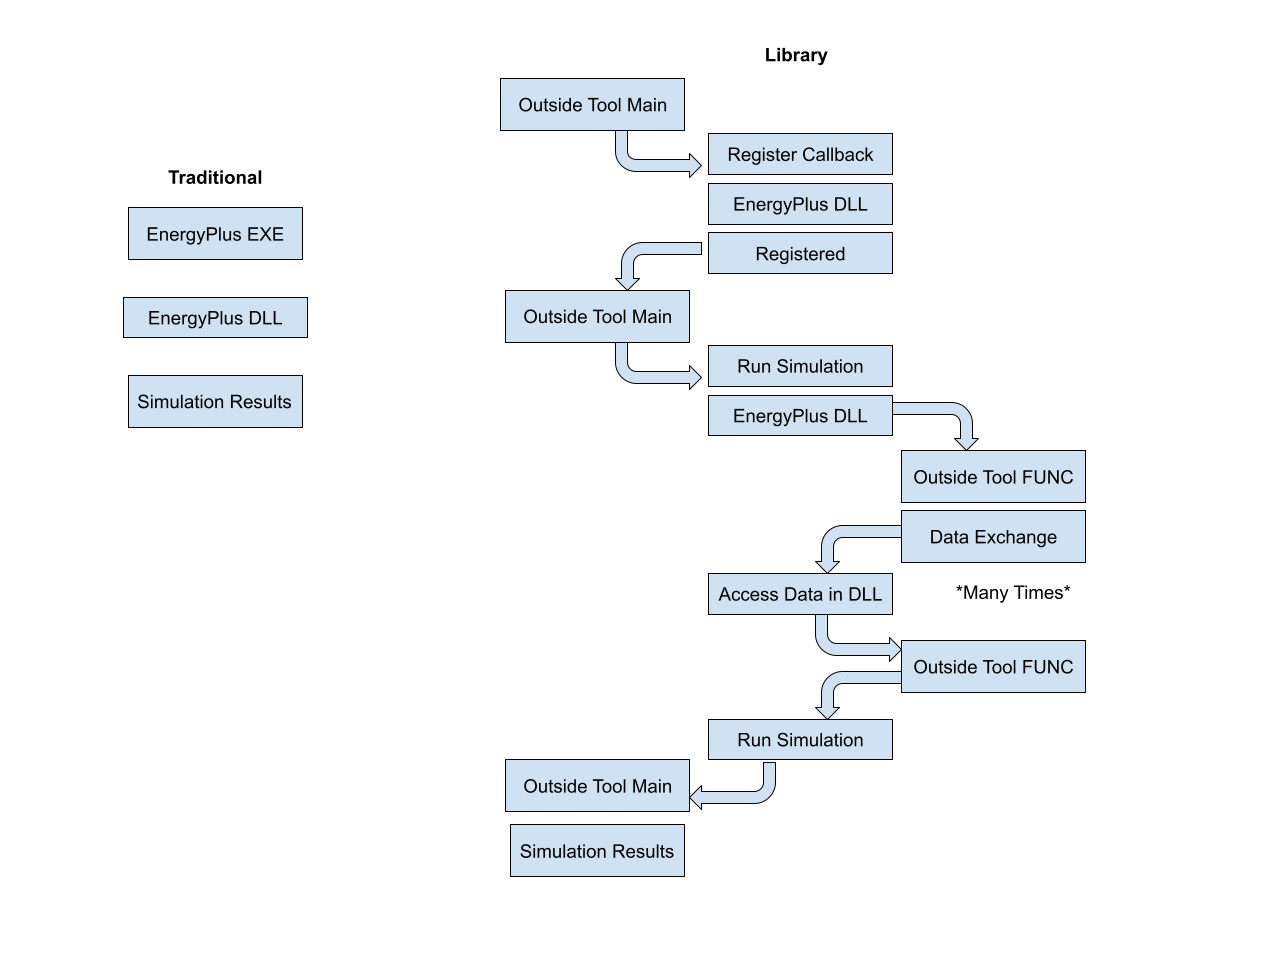
\includegraphics[width=\columnwidth]{images/api_workflows.png}
\caption{EnergyPlus Workflows}
\end{center}
\end{figure}

In the library approach, many new possible calling structures are possible, but they generally follow the same pattern: a client registers functions as callbacks using the runtime API, kicks off a simulation run with the runtime API, and when those registered functions are called back, they can then call back into the library to read and write data using the data exchange API, and perform calculations with the functional API.

The traditional approach will still be the primary calling method for most simulation use cases, as it does not require writing any code to access functionality inside the library.  However, the possibilities opened up by the new library approach are widespread.  Being able to perform data exchange with the simulation from an outside caller unlocks the possibility of connecting with multiple tools at once, keeping tools in lockstep, interfacing with hardware, interfacing with specialized control languages, providing data visualization while a simulation is running, providing simulation feedback while a simulation is running, and more.  The new library approach requires only minimal code, as described in the design section below, but opens the door for major changes in capability.

  \subsection{C API Design}
The details of actually making internal function calls available to clients outside of the compilation unit are not fully described here, as calling into application programming interfaces is standard practice (CITE).  Creating an API that is useful requires careful planning of the functions and classes.  Documenting and conveying the design to clients is equally important as the purpose is to make an interface accessible for users.  In this section, the core C API is described.

EnergyPlus is written in the C++ programming language \cite{Stroustrup1995}.  Exposing a C++ API is possible, but exposing a C API results in a more accessible API for more programming languages, primarily Python.  With the C API layer in place, a Python layer is easily built on top of it for accessing the API.  With the C and Python APIs in place, clients can write C++, C, or Python code that can access EnergyPlus functionality for performing runtime control, data exchange, and functional calculation calls.  In the case of C++ or C, the client code must be compiled and dynamically linked to the EnergyPlus library.  In the case of Python, the EnergyPlus python API layer actually handles the linking process when constructed.  (There could be a diagram from this paragraph)

There are some design guidelines followed when laying out the API.  The actual function names described here should not be considered as official documentation, as the API is subject to change in public versions of EnergyPlus.  Users should access EnergyPlus documentation, examples, and header files to get official API documentation.  However, the important guidelines followed are described here.

In standard practice, the structure of EnergyPlus code is comprised of variables, classes, and functions.  When classes and methods on those classes are to be exposed through the C API,, each class is exposed with the following process:
\begin{itemize}
 \item A C function is created which captures the construction of the class instance, returning a pointer to that instantiated class.  The function should accept all arguments necessary to create an instance of the underlying C++ class.
 \item A C function is created which captures the destruction of the class instance, accepting only a pointer to the instance to be destructed.
 \item A C function for each relevant member variable on the class, with one method for writing and one method for reading where appropriate.  
 \item A C function for each relevant method on the class, with arguments that can be translated to the arguments in the C++ function.
\end{itemize}

An example of this is the glycol routines.  Consider the glycol class in EnergyPlus, and how it is exposed via API functions.

\lstset{language=c}
\begin{lstlisting}
// C++ Glycol Class
struct GlycolAPI {
    ...
    FloatType specificHeat(Real64 temperature);
    FloatType density(Real64 temperature);
    FloatType conductivity(Real64 temperature);
    FloatType viscosity(Real64 temperature);
};

// C API
typedef void * Glycol;
Glycol glycolNew(const char* glycolName);
void glycolDelete(Glycol);
FloatType glycolSpecificHeat(Glycol, Real64 temperature);
FloatType glycolDensity(Glycol, Real64 temperature);
FloatType glycolConductivity(Glycol, Real64 temperature);
FloatType glycolViscosity(Glycol, Real64 temperature);
\end{lstlisting}

In this interface from the core C++ code to the C API, appropriate C types are used in place of C++ standard library types, such as character pointers in place of standard strings.  In addition, to ensure floating point consistency, the internal floating point type used when compiling EnergyPlus is exposed on the C header so that the API, and code built against the API, can use the same floating point type declaration.  Static functions are exposed in a similar fashion, with thin wrapper functions that only communicate in C data types.

The runtime and data exchange APIs are developed similarly, creating thin wrapper functions in C and mapping data in and out of the interface.  There is one notable caveat about data exchange variables: sensor data must be requested prior to initiating a simulation.  During an EnergyPlus simulation, many thousands of output variables can be instantiated and potentially reported.  To avoid a huge memory penalty at runtime, only the requested variables are actually instantiated and available.  This is straightforward in the traditional use case because the input file is available for interpretation at the beginning of the simulation, and all required output variables are already known.  In the library use case, a sensor variable handle may not be retrieved until the simulation is well underway.  To avoid having to track the full potential set of variables, the client should request the variable by name prior to making a call to execute the simulation.  A minimal example is provided here which demonstrates the usage of all three API categories, including the use of requesting an output variable prior to executing the simulation.  

\lstset{language=c}
\begin{lstlisting}
#include <EnergyPlus/api/func.h> // Glycol props
#include <EnergyPlus/api/datatransfer.h> // exchange 
#include <EnergyPlus/api/state.h> // EnergyPlus state
#include <EnergyPlus/api/runtime.h> // E+ and callbacks

void afterZoneTimeStepHandler(EnergyPlusState s) {
  int oaDewPointActuator = getActuatorHandle(
    s, "Environment", "Weather Data", "Outdoor Dew Point"
  );
  setActuatorValue(oaDewPointActuator , -25);
  int oaTempSensor = getVariableHandle(
    s, "SITE OUTDOOR AIR DRYBULB TEMPERATURE", "ENVIRONMENT"
  );
  float oaTemp = getVariableValue(oaTempSensor);
  Glycol glycol = NULL;
  glycol = glycolNew(s, "Water");
  float specificHeat = glycolSpecificHeat(s, glycol, 23.3);
}

int main(int argc, const char * argv[]) {
  EnergyPlus s = stateNew();
  callbackEndOfZoneTimeStepAfterZoneReporting(
    s, afterZoneTimeStepHandler
  );
  requestVariable(
    s, "SITE OUTDOOR AIR DRYBULB TEMPERATURE", "ENVIRONMENT"
  );
  energyplus(s, argc, argv);
  return 0;
}
\end{lstlisting}

  \subsection{Python API Design}
The addition of a C API brings EnergyPlus out of the dark from being a closed off simulation engine to become an interactive library.  This C API alone opens the door for many new applications of EnergyPlus. However, the accessibility and usability of this enhancement can be expanded into a massive set of new possibilities by making the API accessible through the Python programming language and ecosystem \cite{Rossum}.  Adding a Python API enables clients to generate script based workflows utilizing EnergyPlus as well as a wealth of packages and libraries available in Python repositories online.

The EnergyPlus Python API layer is written in pure Python and communicates with EnergyPlus through the now established C API layer.  These capabilities are built-in to the Python standard library, and as such the lower-level details of accessing the C API are concealed from users.  For users consuming the Python API layer, the experience is akin to using any other pure Python package.

Python is an object oriented language, and Python users are accustomed to utilizing libraries which are object oriented.  As such, the EnergyPlus Python API layer is also object oriented.  Each API “type” described above in the C API section (functional, data exchange, runtime) has an accompanying Python class.  Within each class, members and methods provide access to different elements of the API.  There is a single, highest level, class which provides access to all API types and subclasses.  This class (“EnergyPlusAPI”) is defined within a Python package called “pyenergyplus”, that is packaged with EnergyPlus, is effectively a scope for all Python API calls.  The API layer is fully documented, but a pseudocode representation can be described here.  The highest level class contains member variables that capture the three API types.  These, in turn, also contain methods and member variables which are equivalent to the C API methods.  For example, the functional API contains a method called glycol which requires a valid EnergyPlus state instance plus the name of the glycol to construct as function arguments.

Once again, the actual names of the methods and classes provided here are subject to change, and should not be considered documentation of the official API, only a description of how the API was developed.  With this in mind, consider the following example of using the Python API layer to access EnergyPlus:

\lstset{language=python}
\begin{lstlisting}
from pyenergyplus.api import EnergyPlusAPI

def time_step_handler(s):
  outdoor_temp_sensor = api.exchange.get_variable_handle(
    s, "SITE OUTDOOR AIR DRYBULB TEMPERATURE", "ENVIRONMENT"
  )
  dew_point_actuator = api.exchange.get_actuator_handle(
    s, "Environment", "Weather Data", "Outdoor Dew Point"
  )
  api.exchange.set_actuator_value(
    s, dew_point_actuator, -25
  )
  oa_temp = api.exchange.get_variable_value(
    s, outdoor_temp_sensor
  )

api = EnergyPlusAPI()
s = api.state_manager.new_state()
api.runtime.callback_end_zone_timestep_after_zone_reporting(
  s, time_step_handler
)
api.exchange.request_variable(
  s, "SITE OUTDOOR AIR DRYBULB TEMPERATURE", "ENVIRONMENT"
)
api.runtime.run_energyplus(s, sys.argv[1:])
glycol = api.functional.glycol(s, "water")
cp = glycol.specific_heat(s, 23.5)
\end{lstlisting}

With less than 30 lines of (verbose) Python code, a client can access the runtime portion of the API to register a callback function, request and access variable data and set an actuator value, and also access the functional API to calculate the specific heat of a glycol.  This is a minimal--and naive--example of using the API, but demonstrates the accessibility of the API.

 \section{Python Plugins}
The previous sections of this document have focused on the development of APIs to be called from outside tools into EnergyPlus, with the focus of controlling, accessing, and modifying a simulation.  A simultaneous and related effort was made to allow EnergyPlus to simply call out to execute Python scripts at runtime.  This methodology is termed Python Plugins for EnergyPlus.  To users familiar with EnergyPlus and the traditional EMS system, this is essentially an alternative EMS system which uses external Python scripts instead of the IDF-based user defined Erl language scripts.

In the Python Plugin system, EnergyPlus is driving the process, it is not being called as a library from a separate script or tool.  However, these user defined Python plugins can be specified to be called from the same calling points as made available for library calls.  The difference is simply that EnergyPlus is calling out to the Python plugin, rather than the Python code calling into EnergyPlus.  As such, EnergyPlus is the driving program, and must interpret user defined Python code.  To handle this functionality, EnergyPlus is linked to the Python interpreter library.    Internally, EnergyPlus calls out to the user-defined plugin at the desired calling points, and the plugin can then do anything a user can do in Python.  Most use cases of the Python Plugin system will then leverage the previous API efforts, and make requests back into the running EnergyPlus API to get sensor data and write actuator settings.  This is similar to how current EMS based functionality can read sensors and write actuator data.

In order to create a standardized method for calling out from any program to a plugin, it is commonplace to create a plugin base class which must be overridden by clients in creating their own plugin derived classes.  This provides a way to clearly define the requirements of the plugin class as well as allow for evolving plugin capabilities over time by creating alternative base classes.  As with the C API access methods described previously, the following listing and examples are not considered official, but rather representative class names and member names.  A representative snippet of the plugin base class is shown here:

\lstset{language=python}
\begin{lstlisting}
from pyenergyplus.api import EnergyPlusAPI
class EnergyPlusPlugin(object):
  def on_begin_new_environment(self, state):
    # called at the begin_new_environment point
  def on_begin_timestep_before_predictor(self, state):
    # called at the begin_timestep_before_predictor point
  def on_inside_hvac_system_iteration_loop(self, state):
    # called at the inside_hvac_system_iteration point
  ...etc...
\end{lstlisting}

A user will create their own class that derives from the EnergyPlusPlugin base class and overrides one, multiple, or all calling point methods.  The user defined class is instantiated once at the beginning of the simulation and the instance is held in memory throughout the lifetime of the simulation.  This is an important feature because the user has the ability to carry data on the class instance and make it available to multiple calling point functions.  This can be used to persist tracking information, historical data, or any other reason.  Throughout the simulation, the user defined class functions will be called at the appropriate times.  Inside the overridden function, the plugin can then call on the EnergyPlus API to perform calculations using the functional API, and exchange data, reading sensors and writing actuators, using the data exchange API.  Once complete, the function must return an integer.  If the function returns a zero, EnergyPlus will continue running based on that successful signal.  If a nonzero value is returned, it is a signal to EnergyPlus that the simulation should abort based on an error condition.  The plugin function can issue warnings and errors through API methods if desired prior to returning the nonzero value, so that the error file is fully populated with information.

The full process to utilize the Python Plugin system consists of the following pieces:
\begin{itemize}
 \item Create a derived plugin as described above which overrides at least one of the calling point methods
 \item Utilize the Python API to make calls in and out of the running EnergyPlus simulation as needed
 \item Declare the plugin in the simulation input file, specifying the Python module name, the class name, and adding any search paths required to find the Python script
\end{itemize}

Graphics:

\begin{figure}
\begin{center}
\label{figure:plugins:plugin_workflow_cropped}
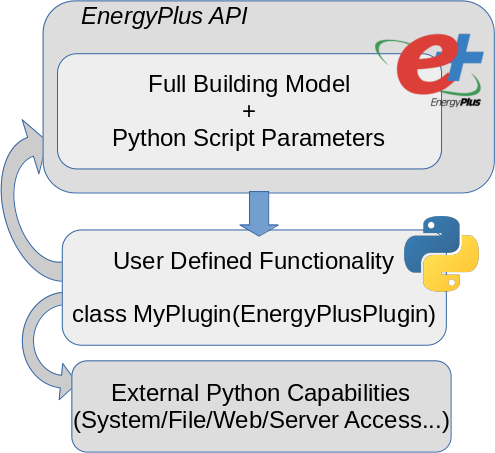
\includegraphics[width=0.7\columnwidth]{images/plugin_workflow.png}
\caption{Plugin Workflow Details}
\end{center}
\end{figure}

\begin{figure}
\begin{center}
\label{figure:plugins:python_ems}
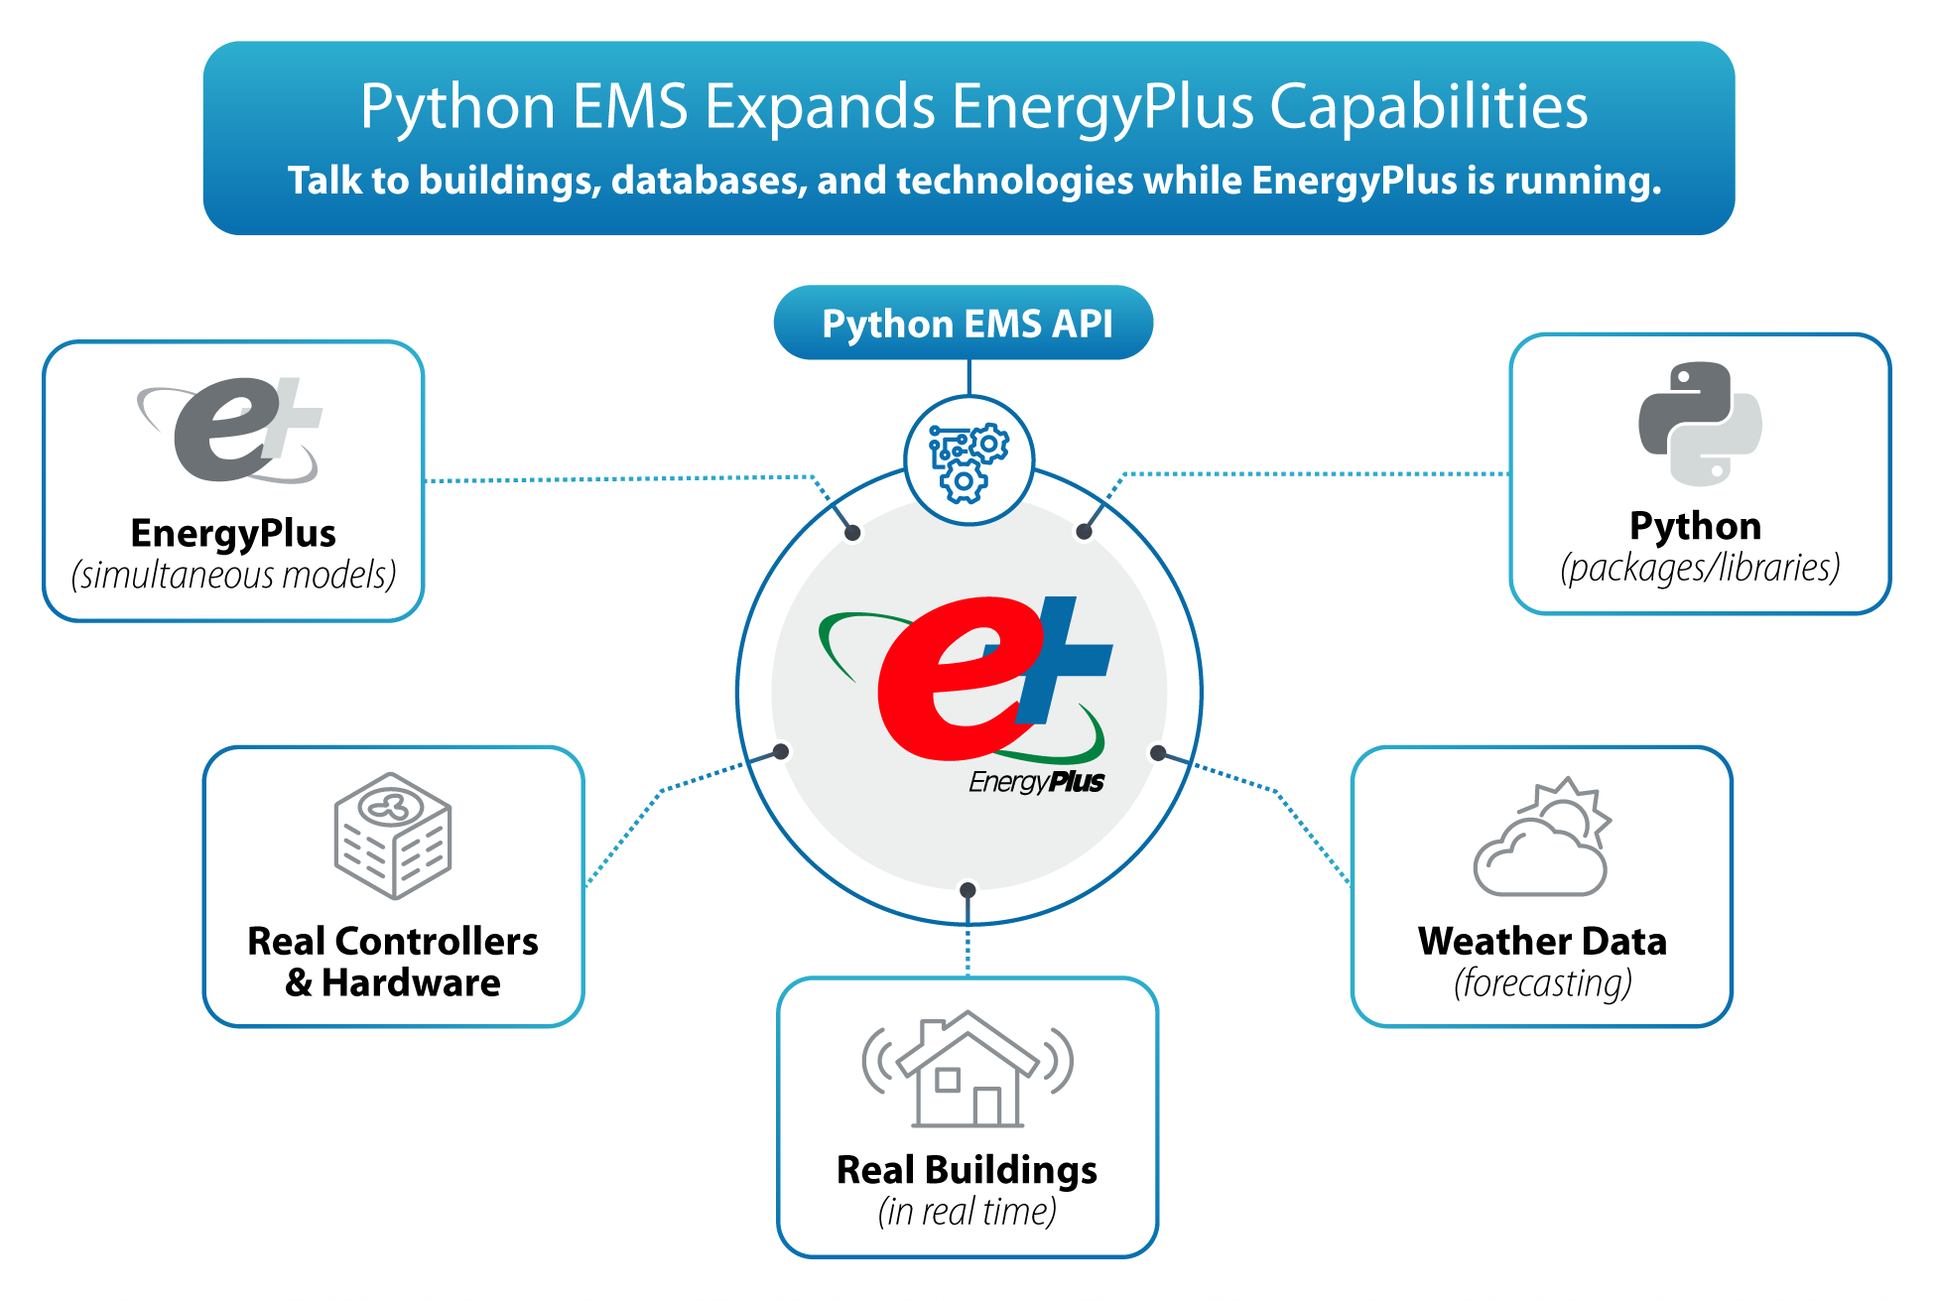
\includegraphics[width=\columnwidth]{images/python_ems.png}
\caption{Python EMS Capabilities}
\end{center}
\end{figure}

 \section{Conclusions}
While the EnergyPlus codebase was made fuly open source years ago, the simulation engine code has been exceptionally difficult for clients to modify and interact with, especially as a library.  There is a wide range of possibilities for clients once the code is made accessible from outside tools.  These possibilities include:

\begin{itemize}
 \item More seamless integration between EnergyPlus and graphical interfaces through runtime calls, which is key for gaining further adoption of EnergyPlus in industry
 \item Lowering the bar for graphical interfaces to be developed by exposing calculation methods that may have previously been duplicated by interface developers
 \item Improving usefulness of EnergyPlus for evaluating novel and complex technologies in a more rapid fashion by allowing implementation of control logic and component models in the Python scripting language
 \item Allowing connection to a wide variety of other configurations, external packages, hardware in the loop and embedding with other simulation tools and languages
\end{itemize}

Frequent concerns/requests when respect to including Python as a dependence are whether or not a client will have to install Python, locking into a Python version, as well as a client’s ability to install third party packages which could be made available to user defined Python code.  While the final implementation is subject to change, the current state of each of these concerns is as follows:

\begin{itemize}
 \item A Python interpreter library along with the Python standard library will be packaged for each supported EnergyPlus platform, and installed as a part of the EnergyPlus program.  This Python package will not interfere with any other system installed versions, and this ensures that a client will not have to install Python separately.
 \item Installing third party packages into a Python configuration is generally straightforward on modern systems when the configuration includes a tool such as Pip (Recursive Acronym: Pip Installs Packages).  A complication arises when the desired package includes “native” binary code, which is different for each platform and must be installed more carefully.  Future plans include putting a version of Pip into the EnergyPlus install to allow inserting packages into the EnergyPlus Python structure, however at the time of writing this has not been completed.
\end{itemize}

 \bibliographystyle{plainnat}
 \bibliography{bibfile}

\end{document}
